\documentclass[12pt, letterpaper, twoside]{article}
    \usepackage[utf8]{inputenc}
    \usepackage{graphicx}
    \usepackage{fullpage}
    \usepackage{pgfplotstable}
    \usepackage{amsmath, amssymb}
    \usepackage{listings}
    
\title{Homework 3 Report}
\date{November 15, 2018}
\author{Sean Kane}

\begin{document}
\maketitle
% \centerline{\textbf{Homework 3 Report}}
% \centerline{\textbf{Sean Kane}}
\section{Problem 1: MNIST Neural Network}


\subsection{System Description}
% Description of all choices made - num of hidden neurons, learning rate, momentum, output thresholds, 
% rules for choosing initial weights, criterion for deciding when to stop training, etc

This neural network is built with 784 input layers - each corresponding to one pixel of a 28 x 28 
image - 150 hidden neurons, and ten output neurons. Each of the ten output neurons corresponded to an
identified number. For example, if the output of the zeroth neuron was a one, this would predict a 
zero, a one at the first neuron meant a prediction of one. A learning rate of 0.01 and an alpha value 
of 0.5 was used for the implementation of momentum. 

During training the output threshold was determined by which neuron had the highest output value of 
over 0.75. If there was not a neuron over 0.75, the outputwas null and the system was trained as if 
it was incorrect. During testing, the predicted neuron was the neuron with the highest value, regardless
of whether it was over 0.75. 

Training of the neural network occurred until one of two conditions was met. The first condition was a 
maximum number of epochs set at 800. This number was chosen because I wanted the machine to see each 
test point an average of ten times, and with a mini batch size of 50 and a test sample size of 4000, 
the epoch on average would be 800. The second condition, which occassionally would cause training to end
before the max epochs, was if the percent change in loss dropped below .01 percent. Percent change was 
measured as:

\[
    PercentChange = \frac{Loss_{N} - Loss_{N-1}}{Loss_{N}}
\]

The percent change was chosen to be a stopping condition because this was seen as a way to prevent overfitting.
If the change in loss was not improving after each iteration, meaning the model was becoming less general
and more specific to the data, then the training needed to stop to keep the model general.

The weights were initialized using the Xavier's initialization method. This is a method to initialize weights
by setting all the weights randomly with a gaussian distribution with a mean of zero and standard 
deviation of one. The value is then multiplied by: 
\[
    \frac{ 1 } { N_i - N_o }    
\]



\subsection{Results}
% Performance of final network on training and test set using confusion matrix.
% Plot time series of error during training saved every tenth epoch
% Testing accuracy: 0.8461 after 297 epochs.
The final network accurately classifed 864 of the 1000 test points for an accuracy of
86.4 percent. The data was trained for 297 epochs before the change in weights appeared to be approaching
overfitting, at which point the training was stopped, the error rate graph was created and the network was
tested against the reserved set. 


% \subsection{Confusion Matrix}

\begin{table}
    \centering
    \pgfplotstabletypeset{confusionmatrix.csv} %[dec sep align, fixed zerofill, precision=0, col sep=space]{confusionmatrix.csv}
    \caption{Confusion Matrix}    
\end{table}

% \subsection{Error Rate Plot}
\begin{figure}
    \centering
    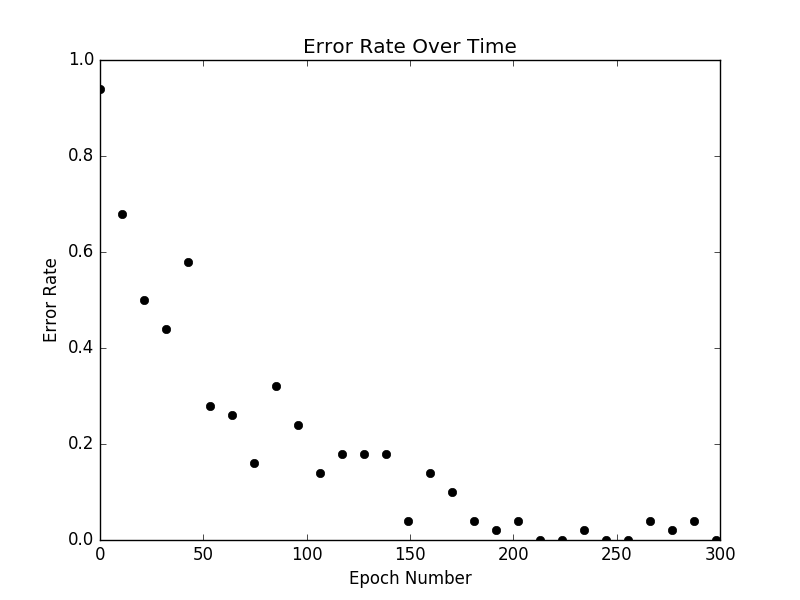
\includegraphics[scale=0.5]{NNErrorRate}
    \caption{Neural Network Error Rate}
    % \caption{Error Rate}
\end{figure}

\subsection{Analysis of Results}
% Describe, discuss, and interpret results you got, and why you think they as as they are.
The error rate can be seen to very clearly drop over time for the entirety of the problem. There were even 
a few mini-batches (of fifty) which were identified perfectly in their epoch. The error rate did settle after
 roughly 150 epochs, and stayed very near to zero 
for the remainder. As can be seen from the confusion matrix, the overwhelming majority of training data 
points were accurately classified. There are some interesting points that can be seen in the matrix, namely 
which ones were the most and least accurate. One, four, seven, and six (in that order), were the most often 
classified correctly. Eight, three, two and nine were the least often classified correctly. In fact, eight
was not classified correctly for even half of the times it appeared. There were several numbers which were 
often mistaken for each other. Seven was most often incorrectly classified as a one, whic seems reasonable, 
but intersetingly, one was rarely misclassified as a seven. Likewise for nine, which was often misidentified
as a seven or four, but four and seven were very rarely misidentified as nines. 

The numbers that were misidentified can be understood if you take into account how similar some of those numbers
can be. A seven can be mistaken for a one if the horizontal line on the top is shorter or not very dark. An eight 
can be mistaken for a nine if at the beginning of the training the feature of the bottom circle (which is present
in the eight and not the nine) is not heavily weighted. 

% \pagebreak
\section{Problem 2: Autoencoder}

\subsection{System Description}
% Description of learning rate, momentum, initial weights, when to stop training.
The system uses 784 input neurons, 150 hidden neurons, and 784 output neurons. The learning
rate was set to 0.1 and the alpha values for the momentum was set to 0.5. The goal of this 
autoencoder was to compress the 784 input neurons to 150 hidden neurons and then have the 
same output as the input, essentially compressing and uncompressing the data value. 
The autoencoder was trained for 1000 epochs or until the percent change in loss was less 
than 0.1 percent. The percent change was defined the same as above. Momentum is calculated 
with the previous epoch's change in weights multiplied by the alpha value and added to the 
current epoch's change in weight. The use of momentum helps prevent the weights from bouncing
back and forth over the goal weights. This helps prevent the weights from drastically changing
because of a single data point, if one point forces the weights highly in another direction
and the next point in the opposite direction using momentum will cancel these out and the final
change in weights is very small. 

% \subsection{Error Graphs}
% Performance of final network on the training set and test set. Two values which 
% should be plotted as two bars side by side. Plot same error in the same way, separated
% by each digit - two bars for 0, two for 1, etc. Plot time series of the overall
% training error during training using the data saved at every tenth epoch. 

\begin{figure}
    \centering
    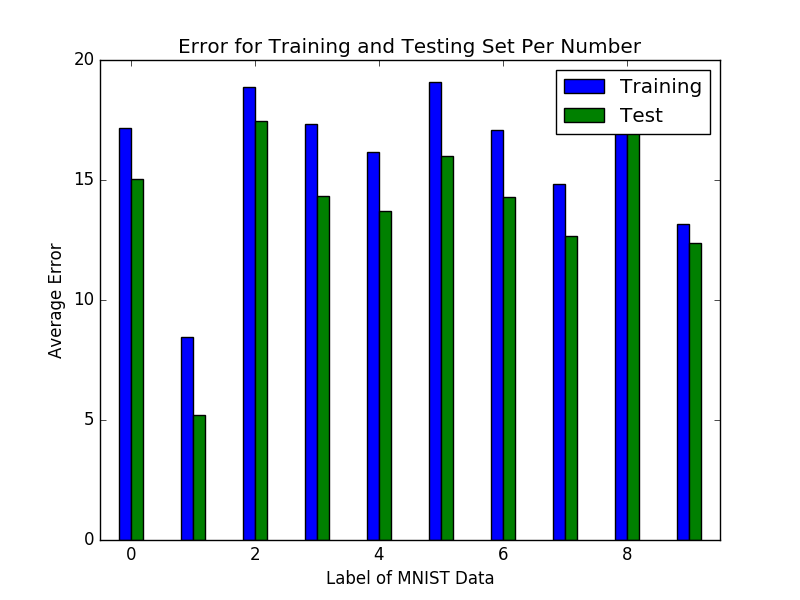
\includegraphics[scale=0.6]{AutoEncoderError.png}
    \caption{Error for each Number}
\end{figure}

\begin{figure}
    \centering
    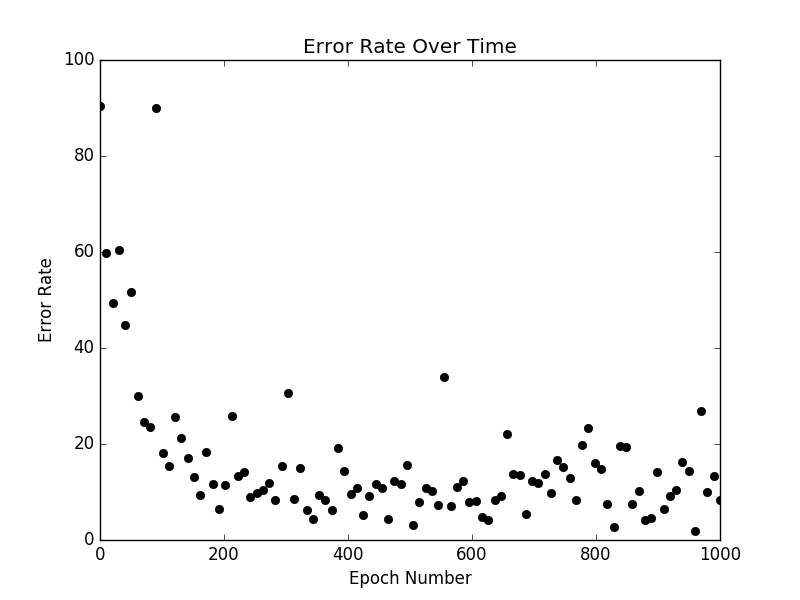
\includegraphics[scale=0.6]{AEErrorRate.png}
    \caption{Error Rate over time}
\end{figure}

% \subsection{Features}
% Plot images for a large number of features, just like data shown in first100.jpg
\begin{figure}
    \centering
    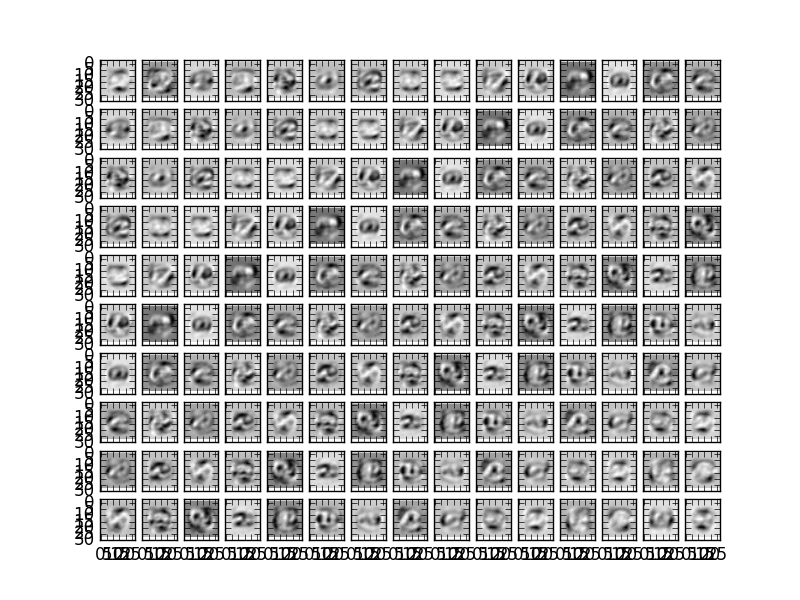
\includegraphics[scale=0.6]{features.png}
    \caption{Features of the Hidden Layer}
\end{figure}

\subsection{Analysis of Results}
% Describe, discuss, and interpret results you got and why you think they are. Comment
% on features you found, and what they suggest. Comment on which digits turned out to be 
% easiest to reconstruct and which ones more difficult, and why you think that happened.

The first plot shows the average error of the testing and training set per each digit.
Overall it can be seen that on average, the autoencoder performed better on the test set 
than on the training set. Visually inspecting the data shows that the difference between
training and testing for each digit is very similar. Of note, it can be seen that the 
autoencoder was better at reproducing certain digits (one, seven, nine, four) than it was 
for other digits (eight, five, two). This might be because the latter group can easily be 
mistaken for each other. Eight and five can be blended together if the difference in contrast
isn't high enough. Whereas a one is distincly individual from each other digit, with the
small exception that a sloppily drawn seven could be seen as a one. This doesn't seem to be 
a likely conclusion because the autoencoder was equally as efficient at reproducing the seven
as it was for the one. 

The second plot shows the error rate over time for the autoencoder. This error function over 
time can be seen to follow the same pattern where it sharply makes corrections in the first
few epochs and then decreases in error are tougher to account for. Over time the error rate
does decrease but not in the same way that the neural network does. This might be because the
reproduction of the 784 neurons from a sample of neurons less than 20 percent is notable more 
difficult than training to recognize digits. 

The final plot shows each neurons trained feature as a grayscale 28x28 image. This was taken
by saving the final weights and plotting the input to each neuron (784 total weights) as a 
28 by 28 pixel image. While none of the features can be exactly seen to represent any of the
handwritten digits, several of them can be determined to exhibit characteristics of individual
digits. For example, the plot at (1, 1) can be seen to have cross arms, which might be indicative
of the number eight if this was highly weighted. Together overlaps of these digits can be used by
the system to decode the compressed input into the full output. 



\section{Program}
All of the files written are python files, so begin by changing main.txt, NeuralNetwork.txt,
dataProcessing.txt, plotFeatures.txt, and AutoEncoder.txt to .py files. dataProcessing.py is a
data processing file which takes MNISTnumLabels5000.txt and MNISTnumImages5000.txt and translates
them into a format easy to import into a python numpy array. NeuralNetwork.py is the main python
file for the neural network, which imports the saved numpy arrays and trains a neural network based
on the preset conditions at the bottom of the script. This file has the option to import a previously
saved set of weights, and to save a final product of weights. AutoEncoder.py is the python file which
performs the auto encoder problem. It also can import weights or save final weights, and after the
training is complete it will trigger plotFeatures.py to plot the saved features of the hidden layer
weights. The graphs requested for this project are saved in the directory that these files are 
saved as .png files. To run this entire project from the command line type: 
\begin{lstlisting}
    $ python3 main.py
\end{lstlisting}

\end{document}